\documentclass{myproject}

\graphicspath{{../Figures/}}

% title setup
\title{\vspace*{-1cm}Numerical Analysis of Burgers' Equation\footnote{Placeholder title!}}
\date{}
\author{
    Andre Gormann\\
    agormann@sfu.ca
    \and
    Ethan MacDonald\\
    jem21@sfu.ca
}

% bibliography
\addbibresource{references.bib}

\renewcommand*{\thefootnote}{[\arabic{footnote}]}

\begin{document}

% title creation
\maketitle
\vspace*{-1cm}

% document 
\section{Introduction\protect\footnote{This entire section has been modified from the content in Chapter 2 of \cite{choksi2022}. Specifically, sections 2.2-2.4.}}

\subsection{The Inviscid Burgers' Equation}

We have elected to study the Burgers' equation, or more correctly, the inviscid Burgers' equation.\footnote{We may decide later on to study the viscous Burgers' equation.} Given $u \in C^1(\Omega)$, where $\Omega \subset \R^{n+1}$ is a domain, the general form is written as
\begin{equation}
    \partial_t u(\bm{x},t) + u(\bm{x},t)\cdot \nabla_{\bm{x}} u(\bm{x},t) = 0
\end{equation}
where $ \nabla_{\bm{x}} $ denotes the gradient with respect to the spatial variable $ \bm{x} \in \R^n $. For pragmatic reasons though, we will be focusing on the $n=1$ case. Then (1) simplifies to
\begin{equation}
    \partial_t u(x,t) + u(x,t)\partial_xu(x,t) = 0.
\end{equation}
There are two key observations to make. The first is that (2) is really a statement about the directional derivative, that is
\begin{equation}
    \nabla u(x,t)\cdot (u(x,t), 1) = 0\footnote{Technically we should be normalizing so that this is a unit vector.}
\end{equation}
so the derivative of $u$ in the direction of $(u, 1)$ is 0 - in other words, $u$ is constant in this direction. This is a consequence of (2) being first-order. While on the surface it may seem problematic that (2) is quasilinear (and so the direction $(u, 1)$ is varied), this does not complicate the finding of an analytic solution. 

\subsection{The Method of Characteristics}

Given data on some curve $ \Gamma \subset \overline{\Omega} $, we are looking specific parametric curves $ (x(t), t) $ which connect points $(x, t) \in \Omega$ to $ \Gamma $. We want these curves to be precisely those which are parallel to the vector $(u, 1)$, that is
\[
    \frac{dx}{dt} = \frac{u(x(t), t)}{1} = u(x(t), t)
\]

Now supposing that $u$ solves (2), let $z(t)$ denote the value of $u$ along a characteristic, i.e. 
\[
    z(t) = u(x(t), t)
\]
Then by the chain rule
\[
    \frac{dz}{dt} = \partial_x u(x(t), t) \frac{dx}{dt}u(x(t), t) + \partial_t u(x(t), t)
\]
but $ x'(t) = u(x,t) $, so
\[
    \frac{dz}{dt} = \partial_t u(x(t), t) + u(x,t)\partial_x u(x(t), t)
\]
which is precisely 0 by (2). Hence, we have the following coupled system of ODEs
\begin{equation}
    \begin{cases}
        x'(t) = z(t) = u(x(t), t) \\
        z'(t) = 0
    \end{cases}
\end{equation}
Integrating the second term, we get that
\[
    z(t) = z_0
\]
for some $ z_0 \in \R $. But $z(t) = u(x(t), t)$, so then $u(x(t), t) = z_0$. This corroborates our findings with (3). Now by integrating the first term, we get
\begin{equation}
    x(t) = z_0t + x_0
\end{equation}
where $ x_0 \in \R $. Evaluating at $t=0$, we have that $x(0) = x_0$. Now assuming we are prescribed some initial condition $u(x,0) = g(x)$, we have that (5) becomes
\begin{equation}
    x(t) = g(x_0)t + x_0
\end{equation}
which are exactly those characteristic curves we initially sought.

\subsection{Interpretation}

For those familiar with the linear transport equation (or advection equation), the physical interpretation of (2) is quite similar; it models the space-time propagation of an initial signal $u(x,0) = g(x)$. The major difference being that the wave-speed is not only not constant - it is proportional to the solution itself (see Figures 1 and 2), and hence can be different along the signal. A consequence of this non-linearity is that the solution to (6) is not always well-defined. Specifically, it can be shown that if $g(x)$ is decreasing on any $E \subset \Gamma$, the solution $u$ will become multivalued at some time $t$ (see Figure 2). This is known as a shock or shockwave. A useful proxy for this behavior is the characteristic curves (Figure 2b\footnote{MATLAB eats the figures' axis labels when downloading this particular image. We have no idea why.}); they converge to the point of discontinuity.

\begin{figure}
    \centering
    \begin{subfigure}{.48\textwidth}
        \centering
        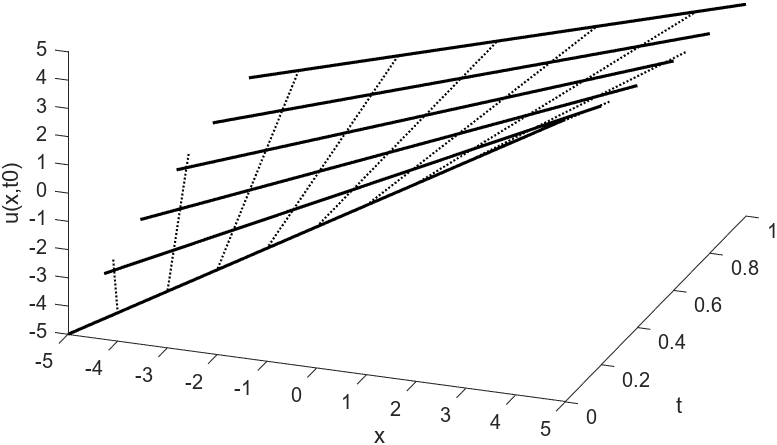
\includegraphics[width=1.0\textwidth]{intro_f1_3d.png}
        \caption{Plot of solution curves at fixed $t\in[0,1]$ with increments of $0.2$.}
        \label{fig:f1_3d}
    \end{subfigure}\hfill
    \begin{subfigure}{.48\textwidth}
        \centering
        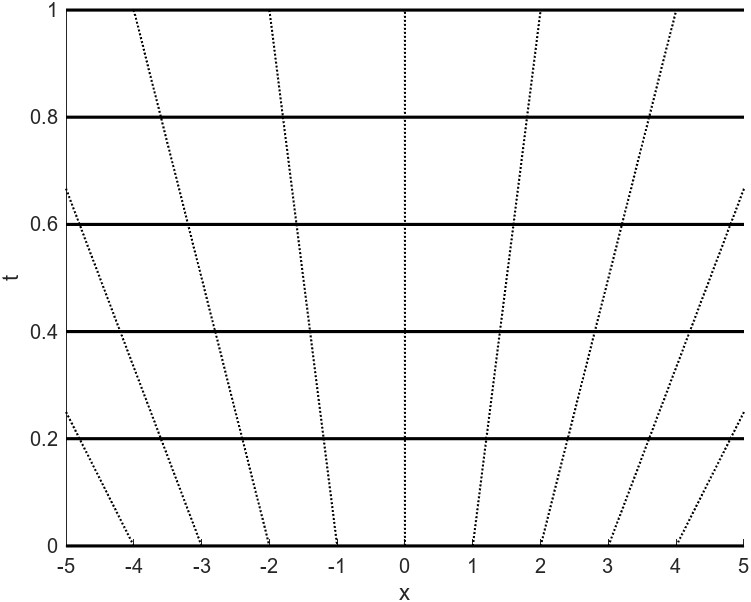
\includegraphics[width=0.75\textwidth]{intro_f1_char.png}
        \caption{Characteristic curves (see (6)) at fixed $x_0 \in [-5, 5]$ with increments of $1$.}
        \label{fig:f1_char}
    \end{subfigure}
    \caption{Solution to (2) with the non-decreasing initial condition $u(x,0) = x$.}
    \label{fig:f1}
\end{figure}

\begin{figure}
    \centering
    \begin{subfigure}{.48\textwidth}
        \centering
        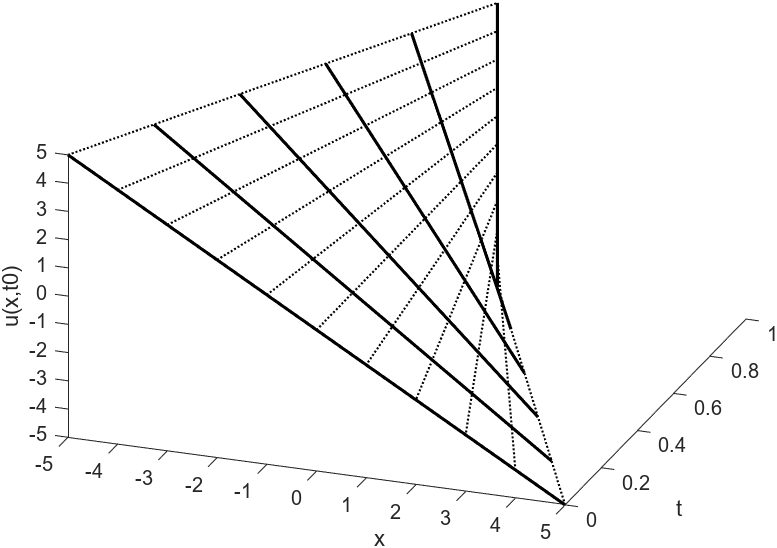
\includegraphics[width=1.0\textwidth]{intro_f2_3d.png}
        \caption{Plot of solution curves at fixed $t\in[0,1]$ with increments of $0.2$.}
        \label{fig:f2_3d}
    \end{subfigure}\hfill
    \begin{subfigure}{.48\textwidth}
        \centering
        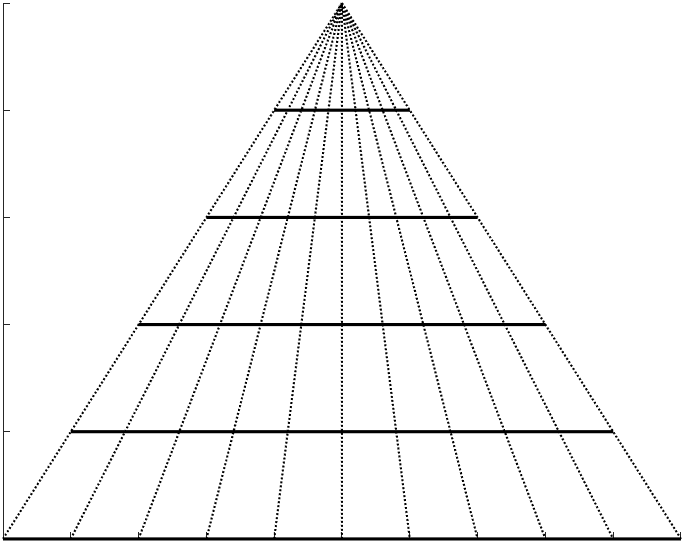
\includegraphics[width=0.75\textwidth]{intro_f2_char.png}
        \caption{Characteristic curves at fixed $x_0 \in [-5, 5]$ with increments of $1$.}
        \label{fig:f2_char}
    \end{subfigure}
    \caption{Solution to (2) with the initial condition $u(x,0) = -x$.}
    \label{fig:f2}
\end{figure}

\pagebreak
\section{Numerical Analysis\protect\footnote{This section has been taken from \cite{learncfd} and \cite{trefethen2001}.}}
Each test problem in this subsection is based upon different choices of $g(x)$ in the IVP
\begin{equation}
    \begin{cases}
        \partial_t{u} + u\partial_x{u} = 0 \quad x \in (a,b), \quad t \geq 0 \\
        u(x, 0) = g(x)
    \end{cases}
\end{equation}
For each test case, we will primarily be using periodic boundary conditions; as the Burgers' equation deals with wave propagation. However, out of curiosity, we will also experiment with Dirichlet, Neumann, and Robin boundary conditions as we see fit. The solutions in for the first two test problems are given explicitly, while the remaining are given explicitly from $(6)$.

\subsection{Test Problems}
\begin{itemize}
	\item \textbf{Riemann Problem}
	
    The Riemann Problem studies the formation of shocks. The initial condition is as follows
	\begin{equation}
		u(x,0) = 
	    \begin{cases}
	      	u_L & \text{if } x < 0 \\
			u_R & \text{if } x \geq 0
	    \end{cases}
	\end{equation}
	where $u_L > u_R$. We will first test different numerical methods for $u_L = 1, u_R = 0$ and then move to problems where $u_L$ is a polynomial and $u_R = 0$.
	
    The true solution is
	\begin{equation}
		u(x,t) = 
	    \begin{cases}
	      	u_L & \text{if } x < st \\
			u_R & \text{if } x \geq st
	    \end{cases}
	\end{equation}
	where \[s = \frac{u_L + u_R}{2}\] is the speed of the shock. This is known as the Rankine–Hugoniot condition.
	
	\item \textbf{Rarefaction Wave}
	
    If we take the Riemann Problem but instead have $u_L < u_R$, a shock will not form. In this case we get what is called a rarefaction wave. From what we understand, the characteristic lines of the true solution become rarified as $t$ increases, meaning the distance between them increases.
	% PERHAPS INSERT A FIGURE OF A RAREFRACTION WAVE IDK HOW THE OTHER FIGS WERE DONE
	The true solution is
	\begin{equation}
		u(x,t) = 
	    \begin{cases}
	      	u_L & \text{if } x \leq {u_L}t \\
			\frac{x}{t} & \text{if } {u_L}t < x < {u_R}t \\
			u_R & \text{if } x \geq {u_R}t
	    \end{cases}
	\end{equation}

	\item \textbf{Sinusoidal Initial Condition}

	We want to investigate our PDE with the initial condition $u(x, 0) = sin(x)$. This should cause a shock to form since $sin(x)$ is sometimes decreasing. We expect similar results for $u(x, 0) = cos(x)$, so we will likely not do much testing with this initial condition. The true solution is
	\begin{equation}
		x(t) = sin(x_0){t} + x_0
	\end{equation}

	\item \textbf{Exponential Initial Condition}

	We want to investigate our PDE with the initial conditions $u(x, 0) = e^x$ and $u(x, 0) = e^{-x}$. We expect no shock for the former since $e^x$ is always increasing. For the latter, we expect a shock since $e^{-x}$ is always decreasing. The true solutions, respectively, are 
	\begin{equation}
		x(t) = e^{x_0}{t} + x_0 \text{ and } x(t) = e^{-x_0}{t} + x_0
	\end{equation}

	\item \textbf{Polynomial Initial Condition}

	We want to investigate our PDE with different polynomial initial conditions. We will test polynomials that are constant, linear, quadratic, etc. until we decide to stop for some reason. In each case, the intial condition will be
	\begin{equation}
		u(x, 0) = g(x)
	\end{equation}
	where $g(x)$ is some polynomial. The true solution is
	\begin{equation}
		x(t) = g(x_0){t} + x_0
	\end{equation}

	\item \textbf{Reciprocal of a Polynomial Initial Condition}

	We want to investigate out PDE with initial conditions of the form
	\begin{equation}
		u(x, 0) = g(x) = \frac{1}{f(x)}
	\end{equation}
	where $f(x)$ is some polynomial of degree at least 1. The true solution is
	\begin{equation}
		x(t) = \frac{t}{f(x_0)} + x_0
	\end{equation}
	These initial conditions should lead to shocks as $g(x)$ will always have a region where it is decreasing.

\end{itemize}

\subsection{Features of Solutions}
At the formation point of a shock, the solution is discontinuous and therefore not differentiable. This leads to a region of poor regularity after the shock. From this, it can be concluded that a numerical solution may blow up due to this region. Something to consider is that for any particular value of $t$, $u(x, t)$ is only discontinuous at the point where the shock occurs. So, $u(x,t)$ will be differentiable to the left and right of the shock, and numerical methods can make use of these derivatives. If instead we have a rarefaction wave, our solution will be smooth. In this case, it can be presumed that numerical solutions will not blow up.

It is also worth mentioning that even though these initial conditions and solutions are potentially only piecewise differentiable, there is still a rigorous way to understand them: distributions. For numerical purposes though, it remains to be seen how relevant this change of scenery would be.

\section{Conclusion}

As aforestated, the Burgers' equation in one spatial dimension will be our primary PDE of investigation. That is not to say that there is no possibility of minor variations such as adding a source/sink term or modifying coefficients (or even major ones such as adding a diffusion term). Since these changes fundamentally alter the solution and interpretation though, they are not a focus. 

We have derived an implicit analytic solution to (2) in the form of (6). Given some fixed $u(x,0) = g(x)$, we can then explicitly solve for the solution $u(x,t)$. If $g(x)$ is decreasing on any interval, then a shock (and hence a discontinuity) is guaranteed. The speed of the shock is characterized by the Rankine-Hugoniot condition. Our first major investigation is studying these phenomena numerically.

% bibliography
\nocite{choksi2022}
\nocite{iserles2009}
\nocite{kutz2013}
\nocite{trefethen2001}
\nocite{learncfd}
\nocite{evans2010}
\printbibliography

\end{document}